\chapter{Methods}
\label{Methods}
\section{Project Overview}
To help complete this Master thesis, I created various tools that would help create the final model outputs. 
The project is divided into three logical parts. 

\subsection{Part 1: Graphical User Interface (GUI) Tool}
The first part involves the development of a GUI tool to create and edit the network topography of interactions. 
This tool allows users to quickly and intuitively define agents, interaction parameters, environmental parameters and setting parameters. 
It provides functionalities for adding, editing, and visualizing nodes and edges, as well as importing and exporting the network structure. 
The tool created a network graph which is then used for part 2 and part 3. 

\subsection{Part 2: Simulation Framework}
The second part focuses on the simulation framework. 
The user provides an ODE model and the network topography as an input to the framework. 
The framework uses numerical solvers to simulate the interactions of the network over time.
As output, the user receives two outputs.
The first output is an array of time values that the solver used to calculate the population count. 
The second output is an array containing the population count of every agent. 

\subsection{Part 3: Analysis and Visualization}
The third part involves analyzing and visualizing the simulation results. 
The user can use a dashboard built using Plotly Dash to interact with the solver and network. 
The user can change parameter, environment values, and setting values on the fly. 
This allows for the user to quickly change parameter values and test different situations. 
The dashboard includes various starter plots that allows for the user to test the model. 

\section{Network Topography of Interactions}
In a microbial environment, there are numerous interactions occurring between agents. 
However not every agent can and will interact with one another.
Based on which agents interact with one another, a network topography can be created, capturing the dynamics of the interactions.
Every node represents a unique agent. 
An edge links agents together if there is an interaction occurring between the agents.  
The network allows for self-loops. 

Each node contains attributes and properties intrinsic to that agent. 
For example, this would include the starting population or concentration, reproduction speed (if any), or death rate (if any). 
Each edge likewise also contains attributes to capture the unique dynamic interactions between the agents. 
This could be the probability for a successful interaction, the burst size of a specific phage-bacteria pair, or the bacteria consumption rate of resources. 
Adding the attributes to the nodes and edges allow for the capture of various interaction dynamics within the context of the community. 
The interactions between the agents can be visualized and edited using a GUI tool. \newline 

A GUI tool has been developed using Python and NetworkX to help aid in the development of this network topography. 
With this tool, a network topography can be created by adding any number of agents of varying type, such as bacteria, phages, or resources.
There is an environment node that is used to store global environmental data, for example the temperature of the system, the pH of the system, washout rate, etc.
There is a settings node that holds information such as simulation length, max timestep, and type of ODE solver to use. 
The attributes of the agents, interactions, and environment can easily be edited using the GUI tool. \newline 

\Cref{fig:ss:initial_startup_GUI_tool} shows the layout of the very simple tool build using tkinter, matplotlib, and NetworkX %TODO: Citation needed. 
Although the button labels are self-explanatory, the buttons allow the user to add exactly 1 node of either type “P” for phage, “B” for bacteria, or “R” for resource and provide a name. 
That is however tedious for large graphs, so the user can add multiple nodes at the same time. 
The newly created node is provided with default parameter values that the user has to provide beforehand. 
This can be done by importing the tool as one would import any other Python package. 
The user provides a base class, extending the class of the tool. 
The user can proceed to override the default implementation of the method that gives the default value. 
It is of course possible to add single or multiple edges at once, remove edges, edit node and edge attributes, and import or export the graph. 

\begin{figure}
    \centering
    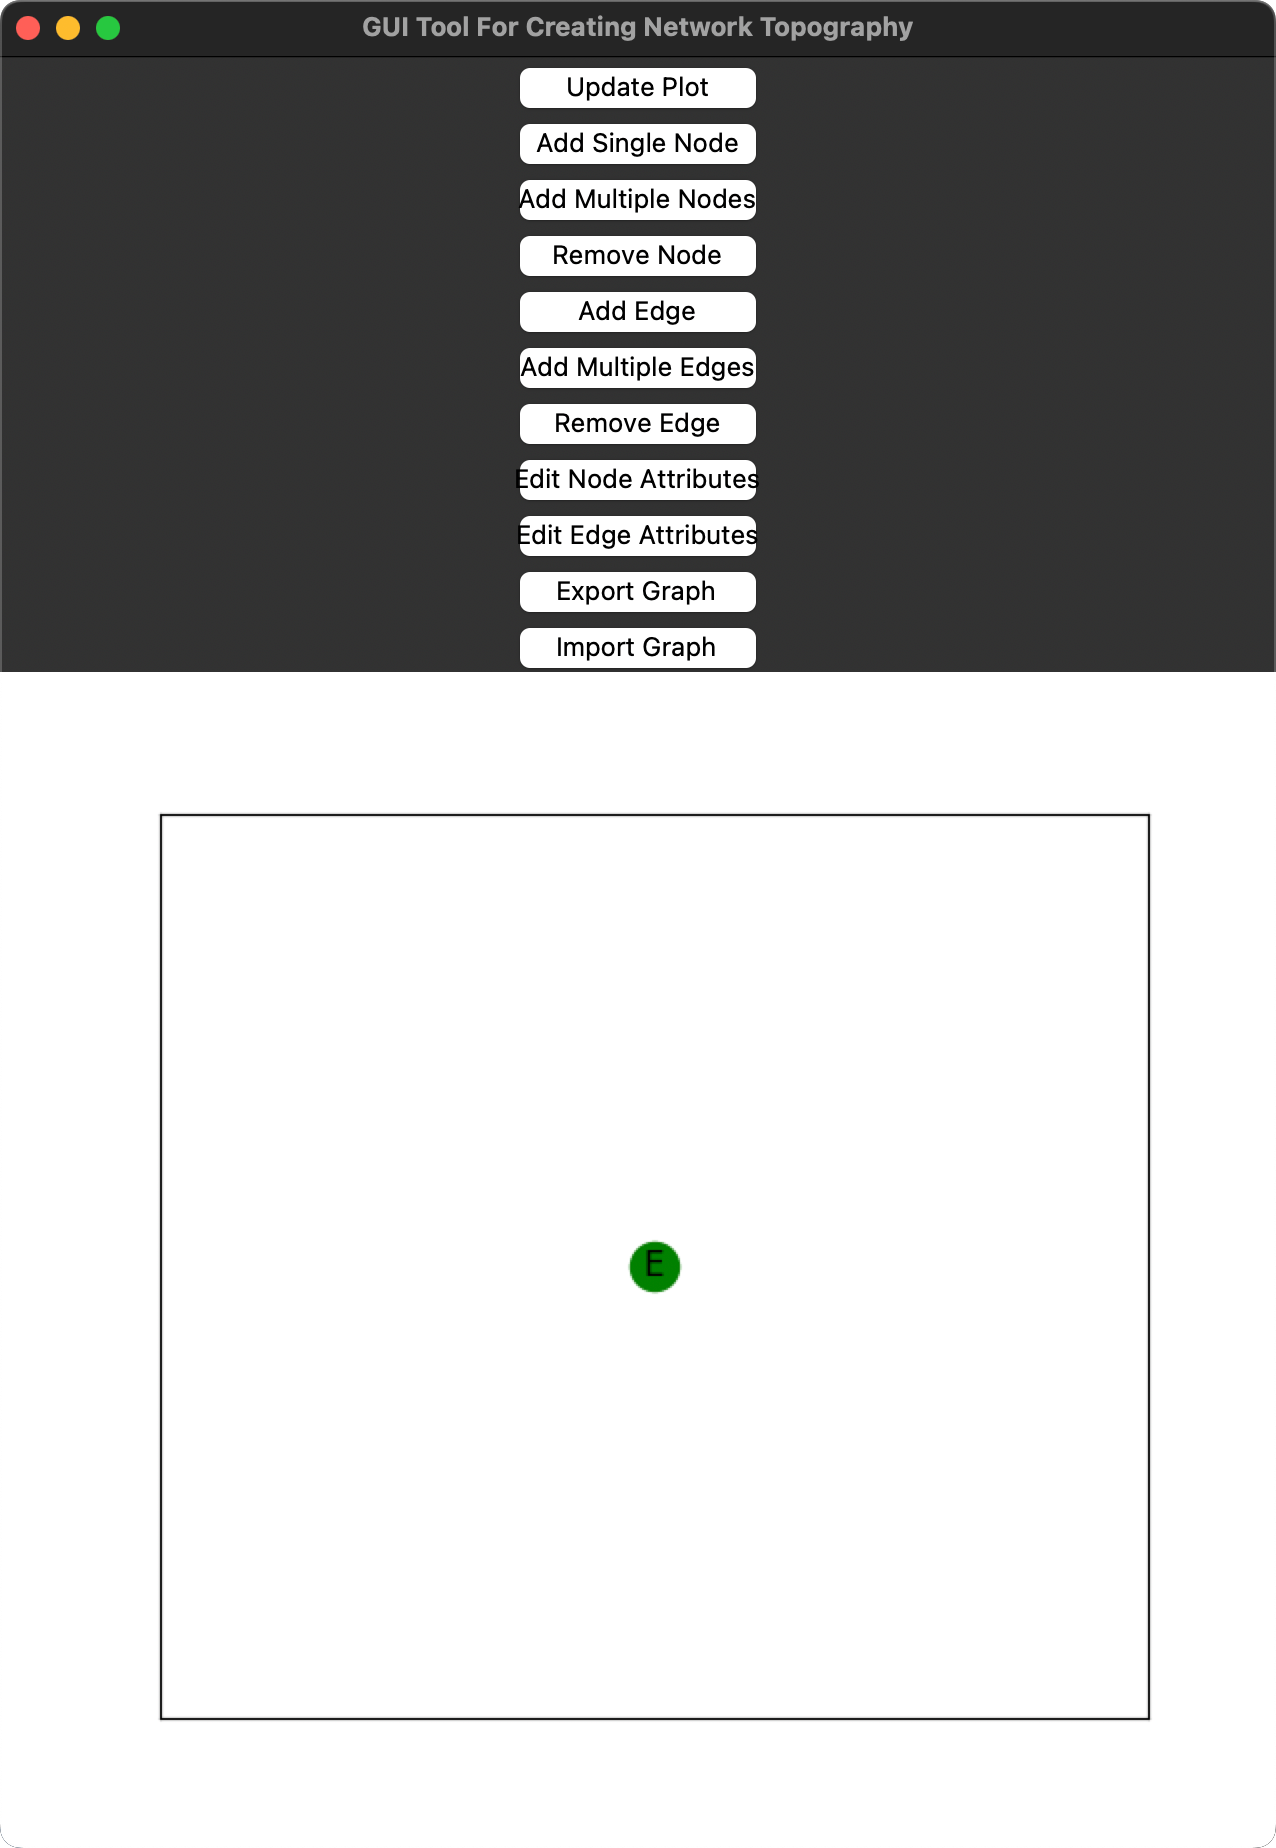
\includegraphics[width=0.5\linewidth]{Screenshots/initial_startup_GUI_tool.png}
    \caption{The GUI tool when you start it up. There are numerous tools that you can use to edit the graph. By default, an environment node holding parameters such as pH and temperature is added. A settings node is added as well, holding settings data to be used for the solver like the type of solver (RK23 or RK45). }
    \label{fig:ss:initial_startup_GUI_tool}
\end{figure}


\begin{figure}
    \centering
    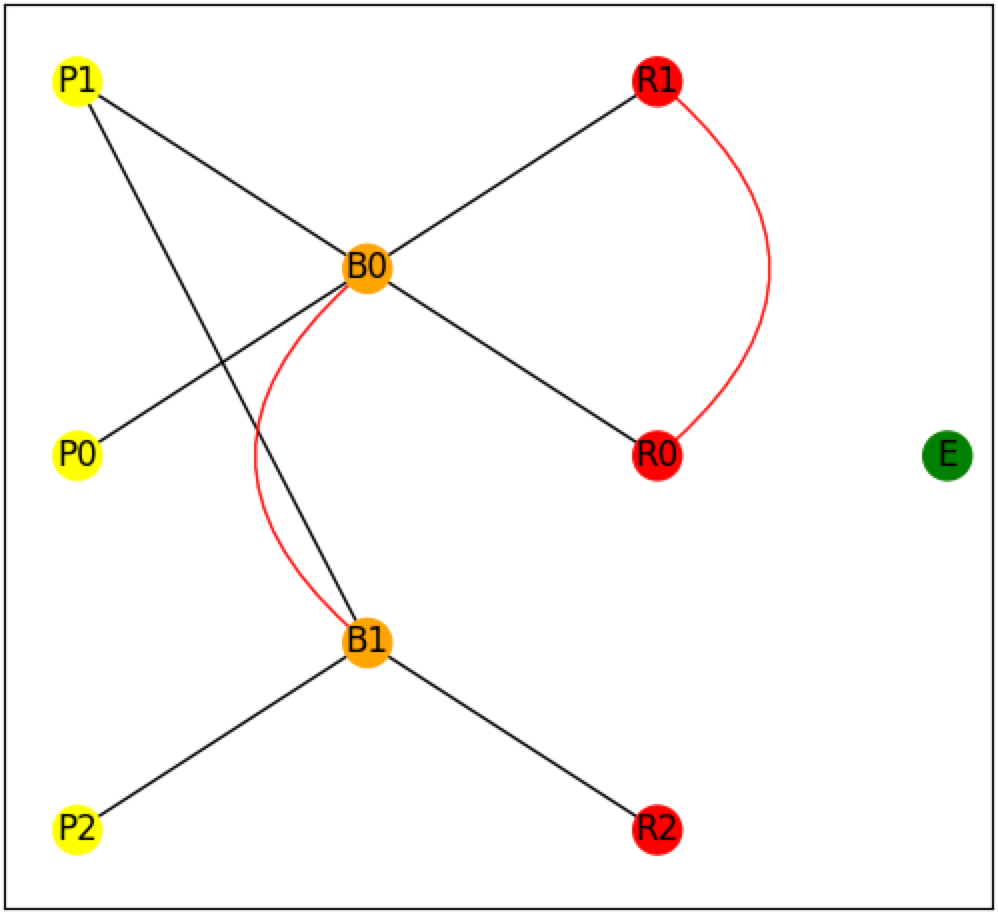
\includegraphics[width=0.5\linewidth]{Screenshots/example_network.png}
    \caption{An arbitrary $3\times2\times3$ network. Phage 0 (P0) interacts/infects bacteria 0 (B0) (and likewise B0 interacts with P0 in some way). P1 infects B0 and B1, etc. Finally, resource 0 (R0) interacts with R1 (an example of this would be a complex sugar degrading into a simple sugar over time). The nature of the interaction needs to be defined and captured in the parameter names, values, and ODE equations. Note: nothing can interact with the environment node.}
    \label{fig:ss:example_network}
\end{figure}
 

\section{Dashboard}
The dashboard allows for the user to interact with the network, the model, and some prebuilt visualizations, and is built into three logical sections. 
The first section allows for the user to edit the network parameters (but not the shape) and setting values on the fly, to quickly iterate through different conditions and to fine tune parameter selection without having to rebuild the network using the GUI tool. 
The first section is closely tied with the second and third section. 
The second section allows for the visualization of the changes in parameter values. 
The user can run a simple run, where the model returns a simple graph showing the population count through time. 
The final section allows for the user to run more advanced analysis, for example by changing multiple parameter values. 

\subsection{Editing Network and Parameter Values}
\label{sec:editing_network_and_parameter_values}
\begin{figure}
    \centering
    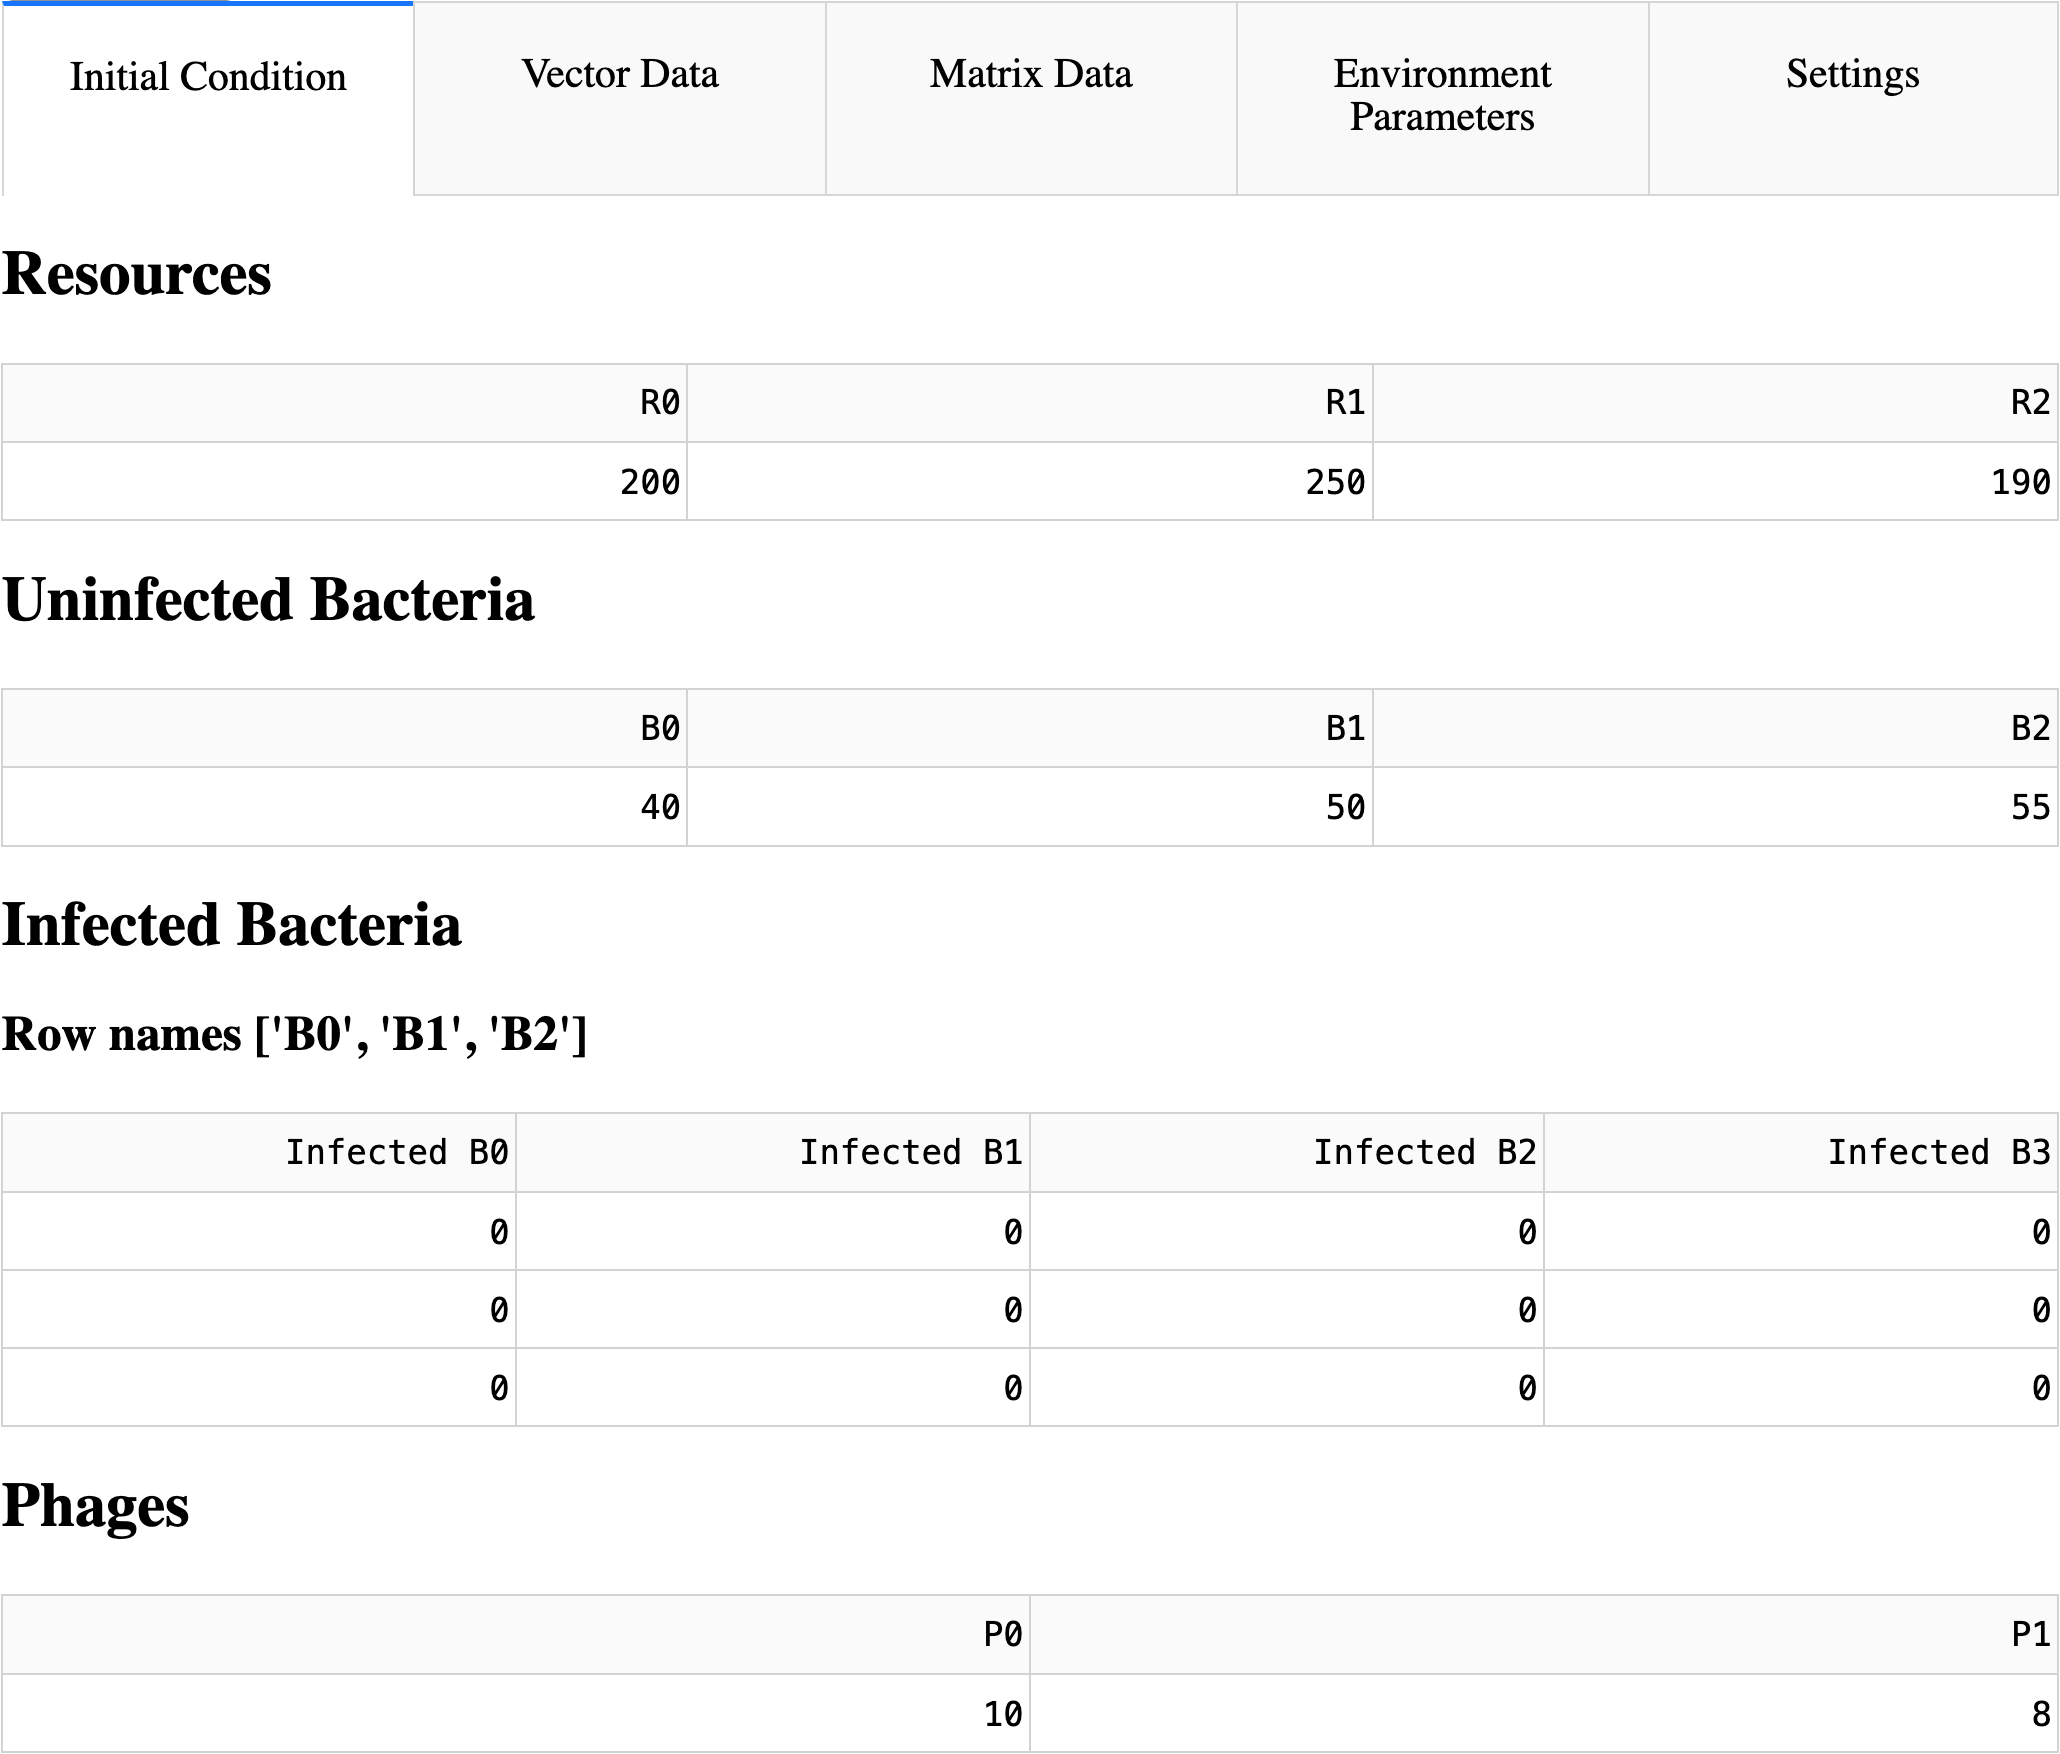
\includegraphics[width=1\linewidth]{Screenshots/DashboardSettings/initial_condition_settings.png}
    \caption{
        The panel where a user can edit the initial conditions of the agents. 
        The columns of each table show for which agent the value corresponds to. 
        A copy of this data is sent to the solver. 
        This instance of the model models a 3 resource, 3 bacteria, and 2 phage system. 
        The bacteria are split into an uninfected and an infected stage. 
        Once infected by a phage, a bacterium will go through four intermediary infection stages before lysing. 
        The infected stages are represented as a matrix, with each row representing a bacterial agent while each column represents the stage of infection. 
    }
    \label{fig:ss:ds:initial_condition}
\end{figure}
\begin{figure}
    \centering
    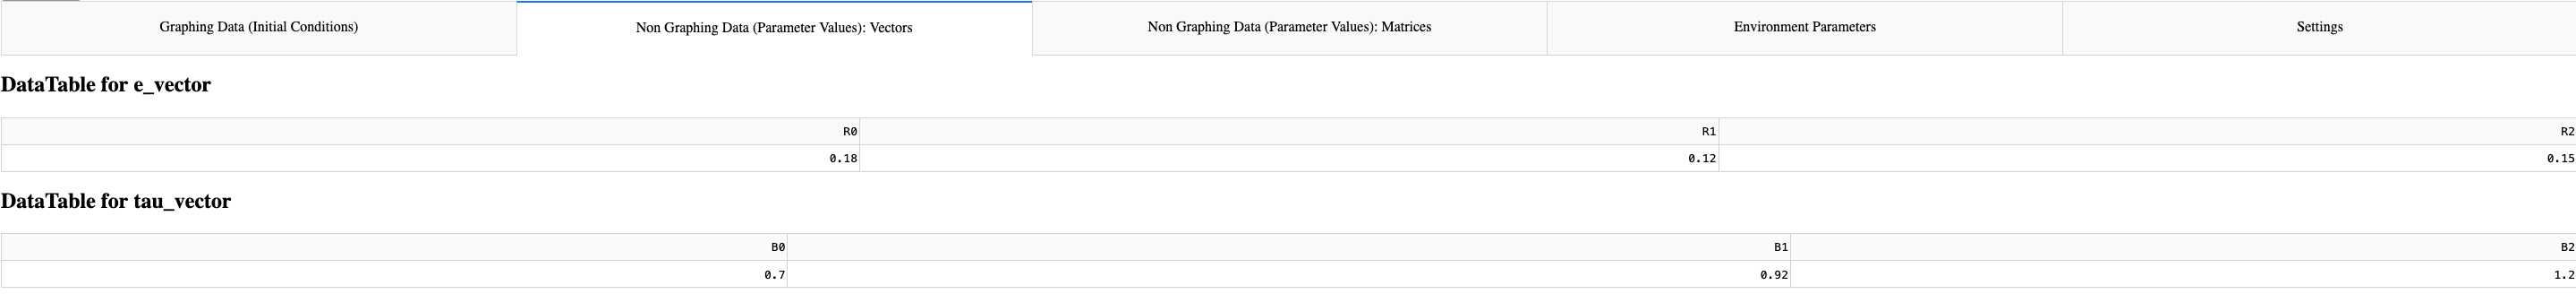
\includegraphics[width=1\linewidth]{Screenshots/DashboardSettings/initial_vector_settings.png}
    \caption{
        The panel where the user can edit the attributes for a given attribute name. 
        This version is specifically used represent the attributes that are associated with nodes, and are represented as a vector. 
        The columns of each table show for which agent the value corresponds to. 
        A copy of this data is sent to the solver.
    }
    \label{fig:ss:ds:vector}
\end{figure}
\begin{figure}
    \centering
    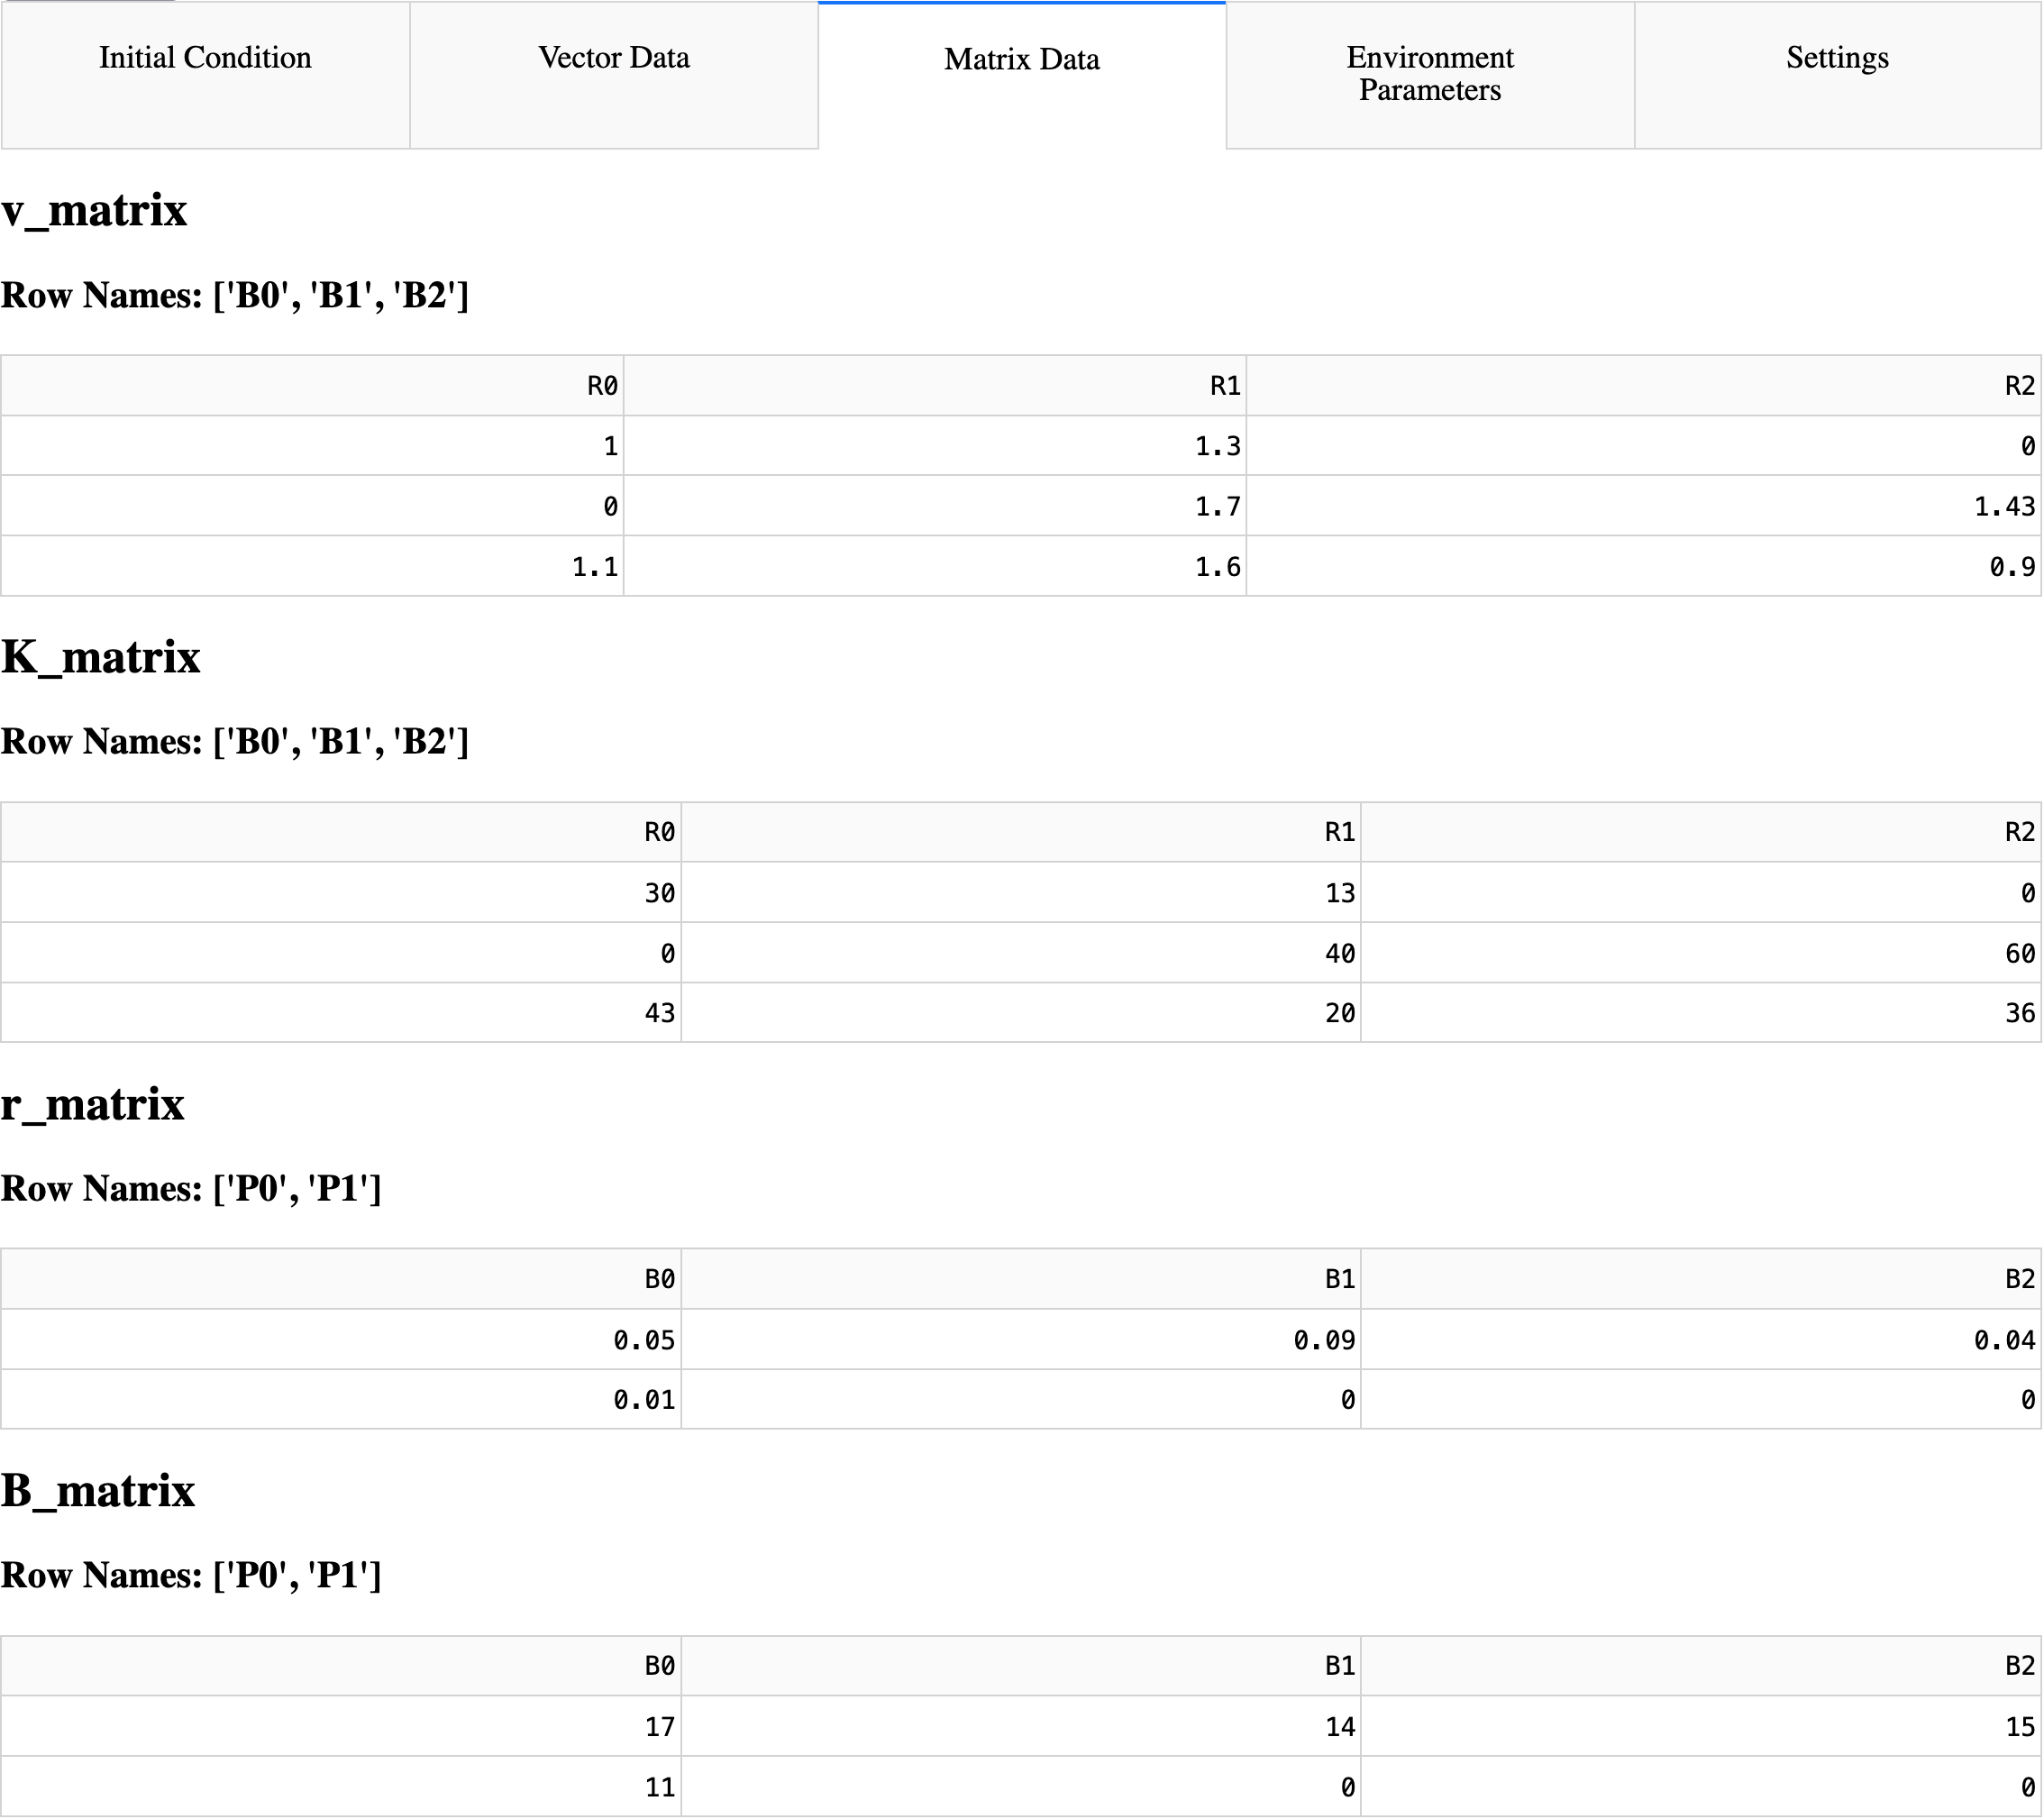
\includegraphics[width=1\linewidth]{Screenshots/DashboardSettings/initial_matrix_settings.png}
    \caption{
        The panel where the user can edit the attributes for a given attribute name. 
        This version is specifically used to represent the attributes that are associated with edges between agents, and are represented as a matrix. 
        The rows and columns of each table show for which agent the value corresponds to. 
        Due to limitations with Dash datatables, the row names can't explicitly be labelled, however text above the table shows the row names. 
        A copy of this data is sent to the solver. 
    }
    \label{fig:ss:ds:matrix}
\end{figure}
\begin{figure}
    \centering
    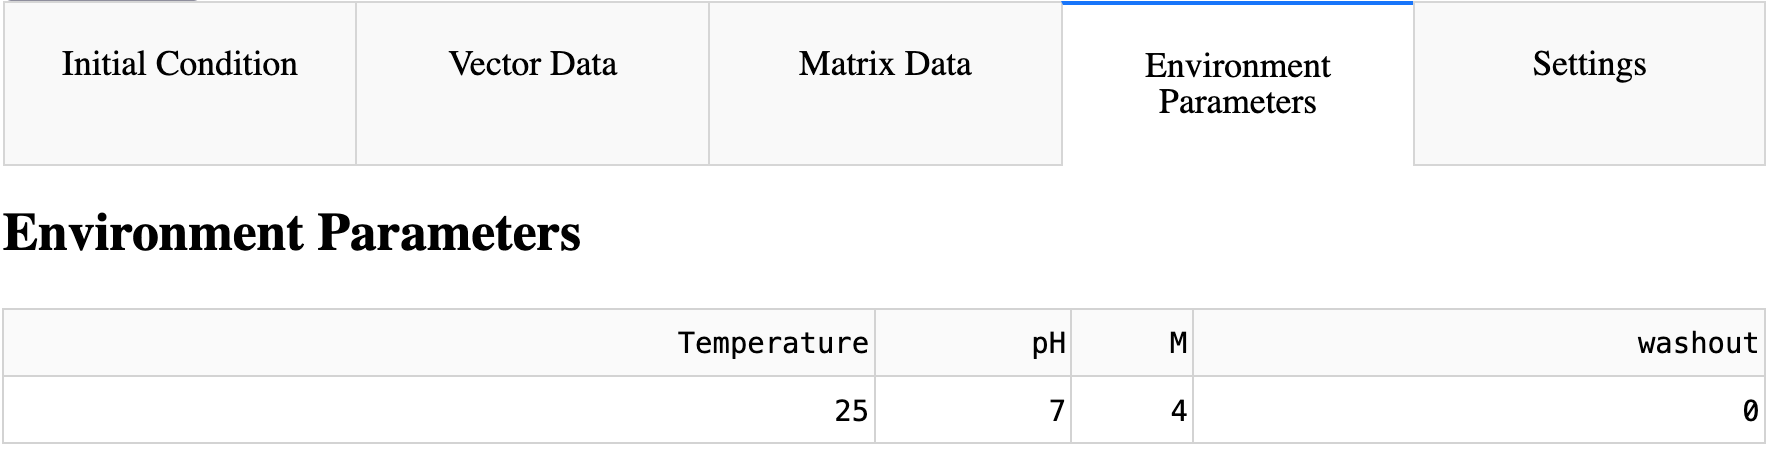
\includegraphics[width=1\linewidth]{Screenshots/DashboardSettings/initial_environment_settings.png}
    \caption{
        The panel where a user can edit the edge attributes the environment settings. 
        Each column represents a single environment parameter. 
        A copy of this data is sent to the solver.
    }
    \label{fig:ss:ds:environment}
\end{figure}
\begin{figure}
    \centering
    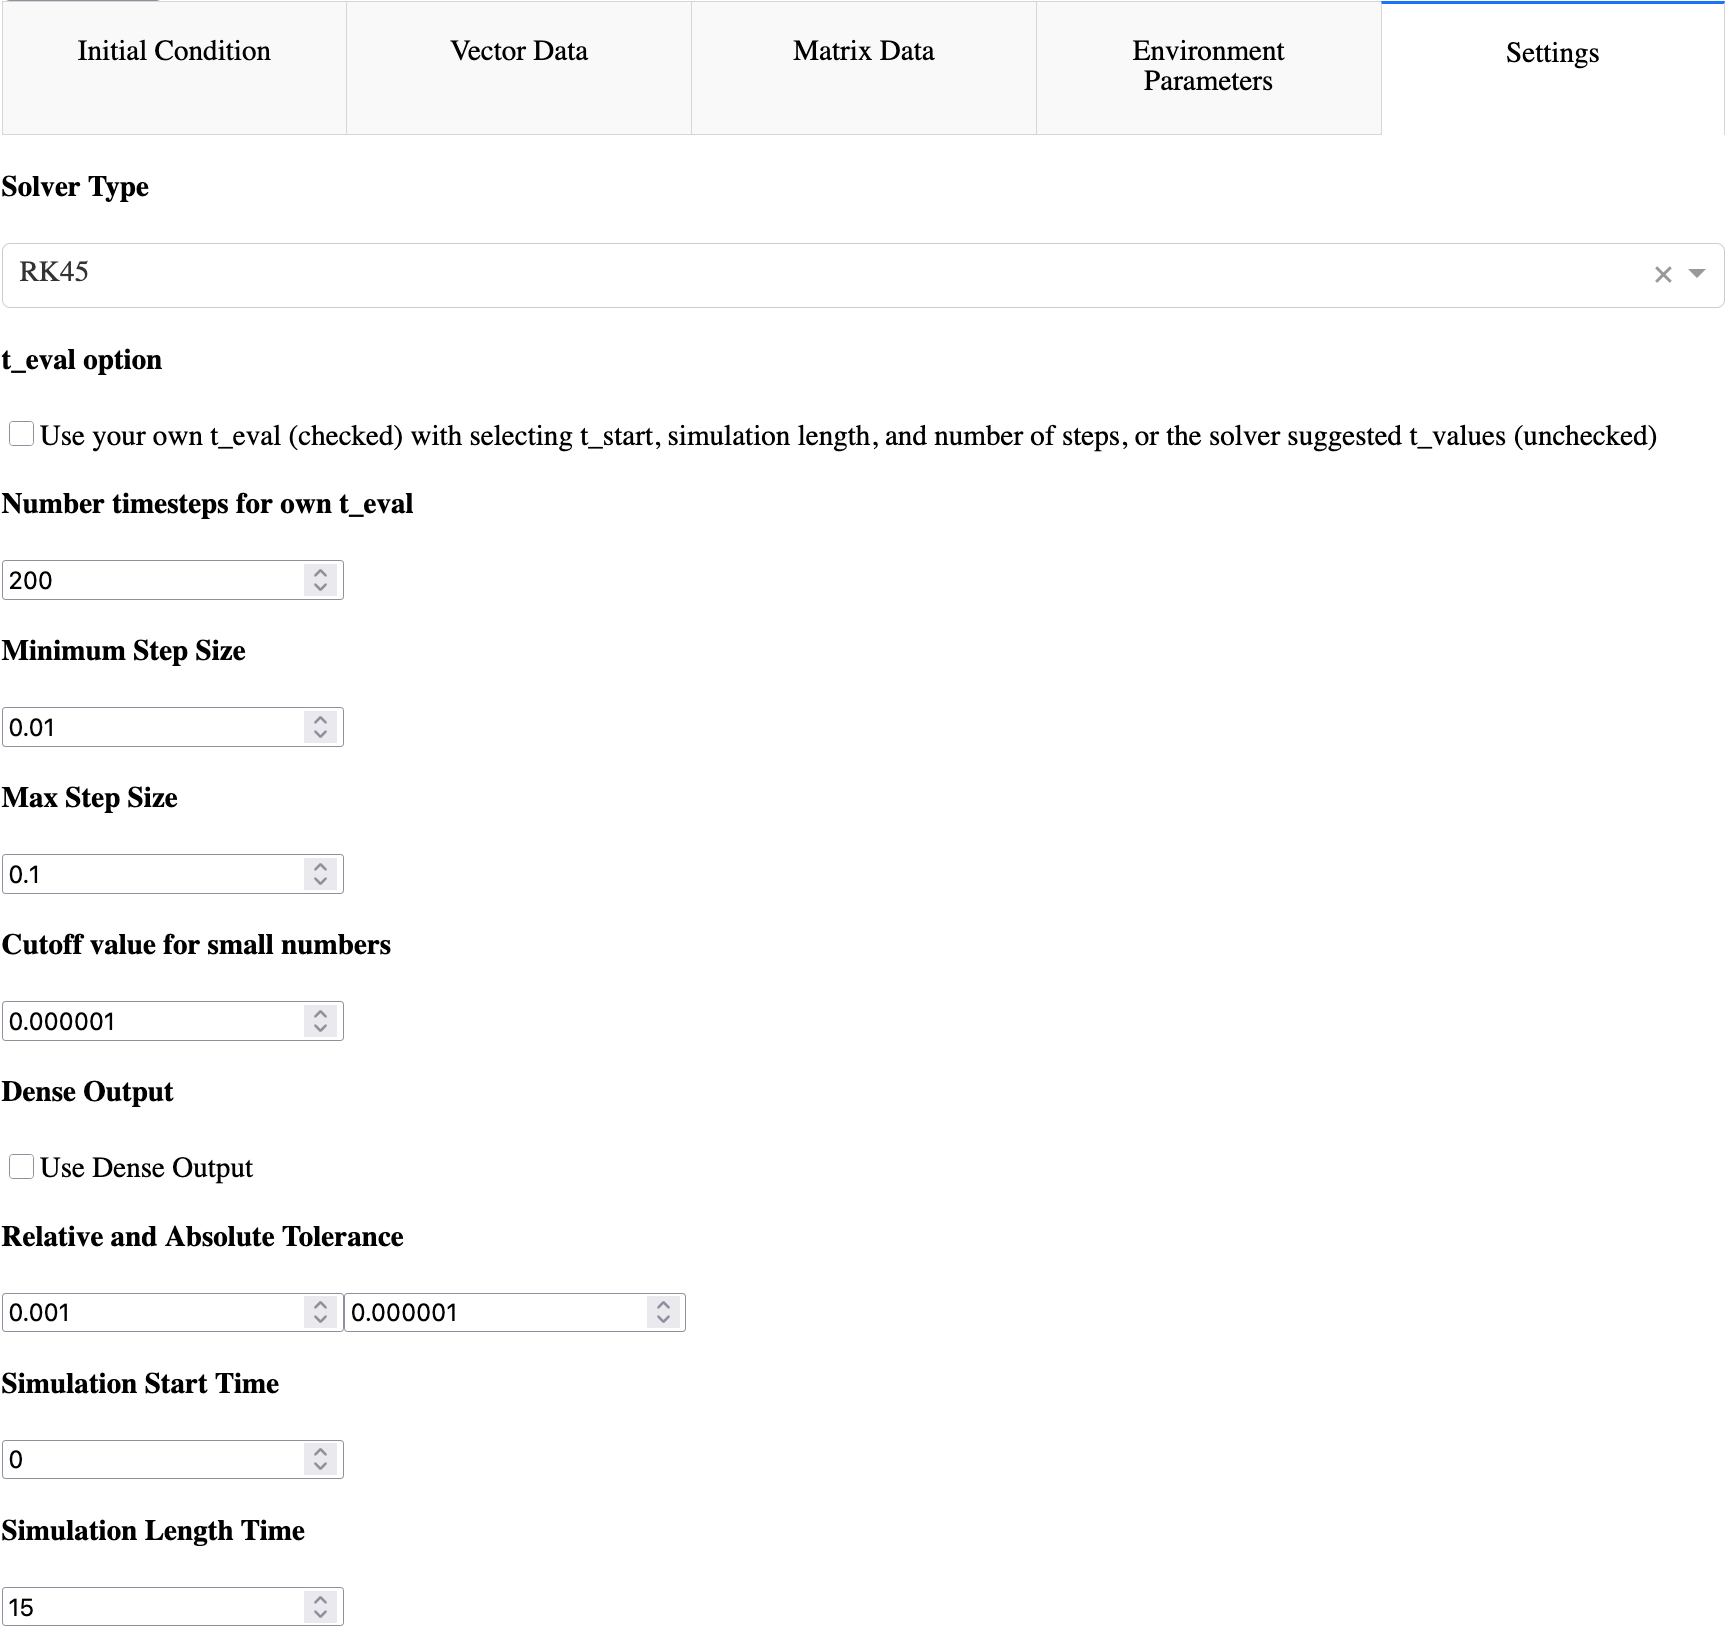
\includegraphics[width=1\linewidth]{Screenshots/DashboardSettings/initial_settings_settings.png}
    \caption{
        The panel where a user can edit the settings of the solver. 
        Various options exist, such as solver type, cutoff value for small values, or tolerances of the solver. 
        A copy of this data is not sent to the solver. 
        The user needs to save the settings, while for the other panels the user does not need to save the changes. 
    }
    \label{fig:ss:ds:settings}
\end{figure}

\subsection{Advanced Visualization and Analysis}
In the advanced analysis section, the user can run different analysis methods to gain a greater understanding of the model. 
The visualizations only support a $1 \times 1\times 1$ model, in order to make the analysis easier for the user, and to make it easier to analyze the visualization. 
These advanced visualizations were created with the mind of understanding a simple network. 
There are five different analysis and visualization methods, and one system where the user can run a large simulation on the whole network and receive an output file containing the raw simulation file data. 
The raw data is stored as a \textit{parquet} file, a tabular-like dataformat, which when combined with Dask (note: not Dash), allows for querying of the data similarly to Pandas. 
Parquet with Dask offers superior performance and data storage solutions that Pandas can't offer. 
Once queried, the user can create their own graphs and plots as they have access to the parameter values used and the raw simulation data. 
\subsubsection{Serial Transfer}
Serial transfer is a method employed by bacteriologist where after a set amount of time, the bacteriologist pipettes a specified amount of media (for example 10ml of liquid) containing bacteria and  nutrients, possibly with phages, and transfers the old media into a solution containing new media. 
At this stage, the bacteriologist can introduce new agents, or re-introduce agents if the agent population or concentration has died out. 
However, usually only resources are added during the transfer process. 
An example would be an experiment starts with 50ml of solution. 
The experiment runs for 24 hours before 5ml is removed. 
Researchers can run various tests, such as using optical density measurements to assess bacterial density in the solution or employing a mass spectrometer to determine the concentration of the resources. 
The 5ml is then re-added to a new solution of 45ml containing fresh resources. 
The effect that this has is tit creates a sort of artificial stable point. 
As the bacteria grow, they consume the resources found in the solution. 
However eventually the resources run out, and the bacteria die out due to a lack of nutrients. 
By introducing new nutrients at set time intervals, the bacteria can regrow and exhibit a semi-stationary behavior. 
\newline 

The implementation of serial transfer is slightly different. 
A user can select a number which will divide the population count of the agents by that number. 
Then the program takes the initial condition values defined for the nutrients the initial condition in \ref{sec:editing_network_and_parameter_values} and adds those values to the nutrients respectively. 
By selecting a checkbox, the values as defined in the initial condition box for phages and bacteria in \ref{sec:editing_network_and_parameter_values} can optionally be added as well. 
As a concrete example, if at the end of a simulation, there are 120 resources remaining, 5000 bacteria, and 1000 phages, and the chosen serial transfer value is 15, then the ending resource, nutrient, and phage value is 8, 333.33, and 66.66 respectively. 
If the initial condition for the resources, bacteria, and phages are 500, 80, and 10 respectively, then if the checkbox is unchecked, the new population count will be 508, 333.33 and 66.66 respectively. 
If the checkbox is checked, the new population count will be 508, 413.33, and 76.66 respectively. 

\begin{figure}
    \centering
    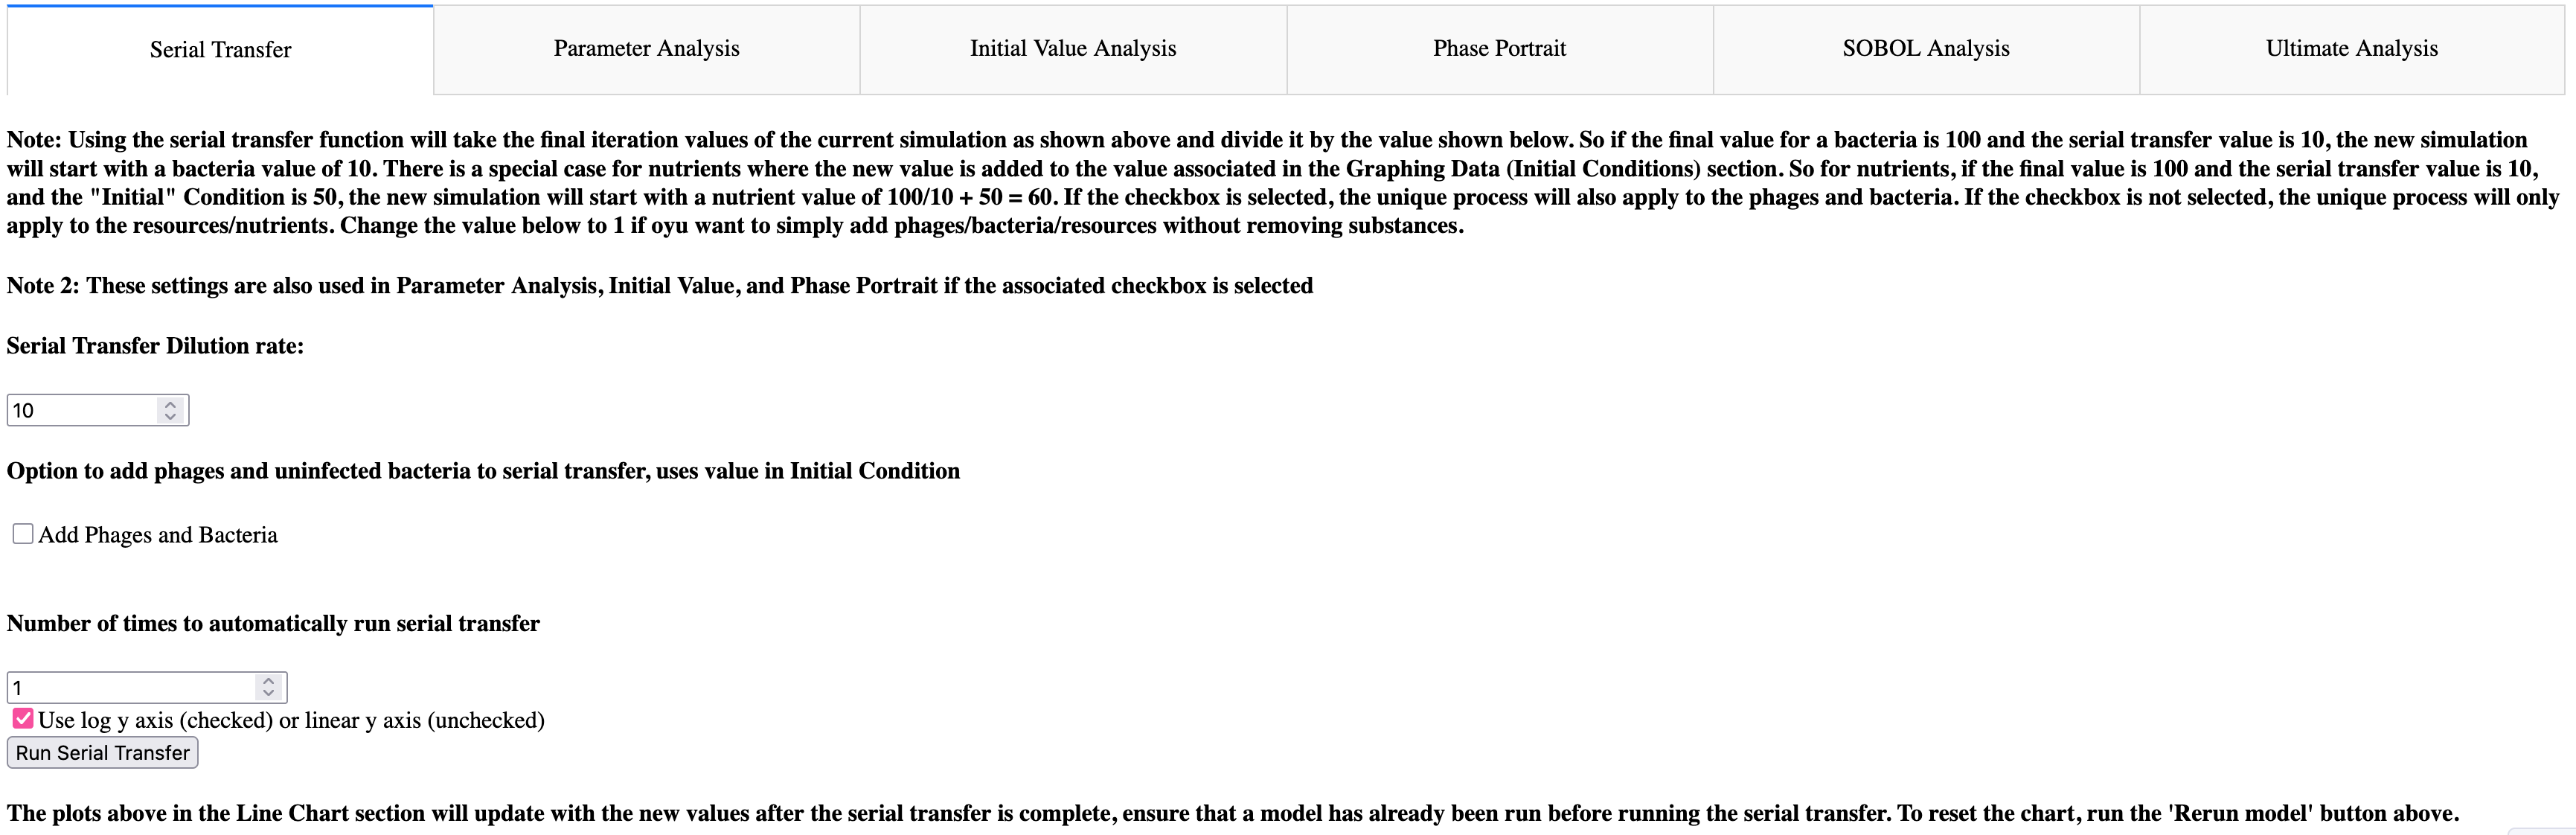
\includegraphics[width=1\linewidth]{Screenshots/AdvancedVisualization/serial_transfer_settings.png}
    \caption{
        The section where the user can set up the serial transfer. To adjust the values added, the user would need to edit the initial condition values. 
    }
    \label{fig:ss:av:serial_transfer_settings}
\end{figure}
\begin{figure}
    \centering
    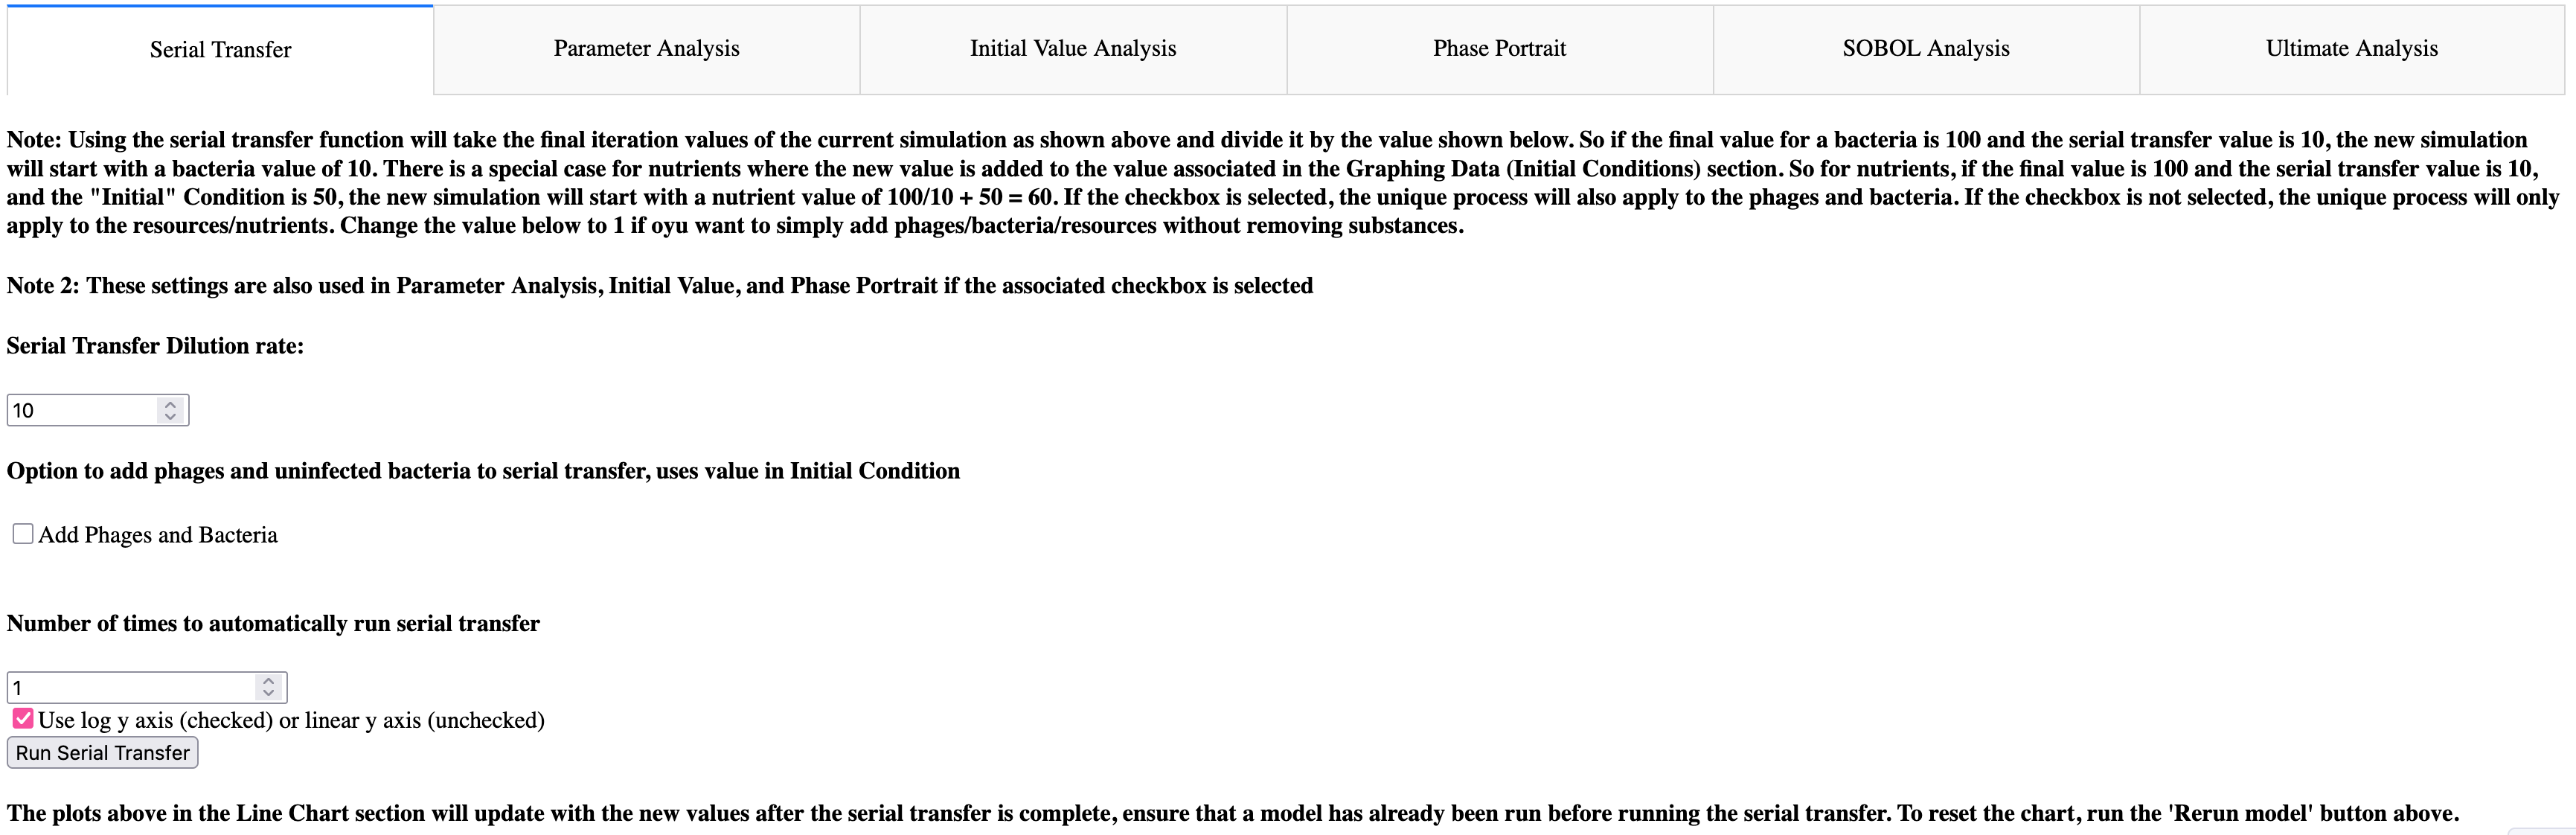
\includegraphics[width=1\linewidth]{Screenshots/AdvancedVisualization/serial_transfer_settings.png}
    \caption{
        Running the serial transfer updates the plot at the top of the page. The simulation initially ran for $t=10$, and completed two serial transfers with a dilution rate of 10. The first transfer was compelted without adding new phages and bacteria. The second transfer was doen with adding new phages and bacteria. 
        The R1 (red) and R0 (purple) resource died out at $t=1.5$ and $t=2.8$ but are reintroduced at $t=10$ as part of the serial transfer process. 
        All bacteria become infected and die out before or at $t=10$. 
        At $t=10$ the phages have a value of roughly 818 and 1078 pre-serial transfer, and have a value of 81.8 and 107.8 post serial transfer. 
        At $t=20$, a second serial transfer occurs where bacteria are reintroduced to the system, and more phages are added to the existing population. 
        The stacked line plots show the absolute and relative distribution of different population groups. 
        The stacked barchart at the bottom shows the final population count of each agent group type at the end of each serial transfer. 
        It might not always be feasible to experimentally determine the population count at each timestep in a lab, hence this graph can be used as a replacement to show the population count at serial transfer time. 
    }
    \label{fig:ss:av:serial_transfer_run2_with_p_b}
\end{figure}

\subsubsection{Parameter Analysis}
\subsubsection{Initial Value Analysis}
\subsubsection{Phase Portrait}
\subsubsection{SOBOL Analysis}
\subsubsection{Ultimate Analysis}